\section{INTERCONNECT System-Level Modelling}
The INTERCONNECT model represents the ring at circuit level using straight waveguides, waveguide couplers, a ring round-trip path, input/through/drop ports, and an optical network analyser. This level is useful for quickly predicting resonant transfer functions and checking how \(n_g\), round-trip length, and coupling coefficients affect FSR, linewidth, \(Q\), finesse, and drop-port power \cite{labmanual}.

\begin{figure}[H]
\centering
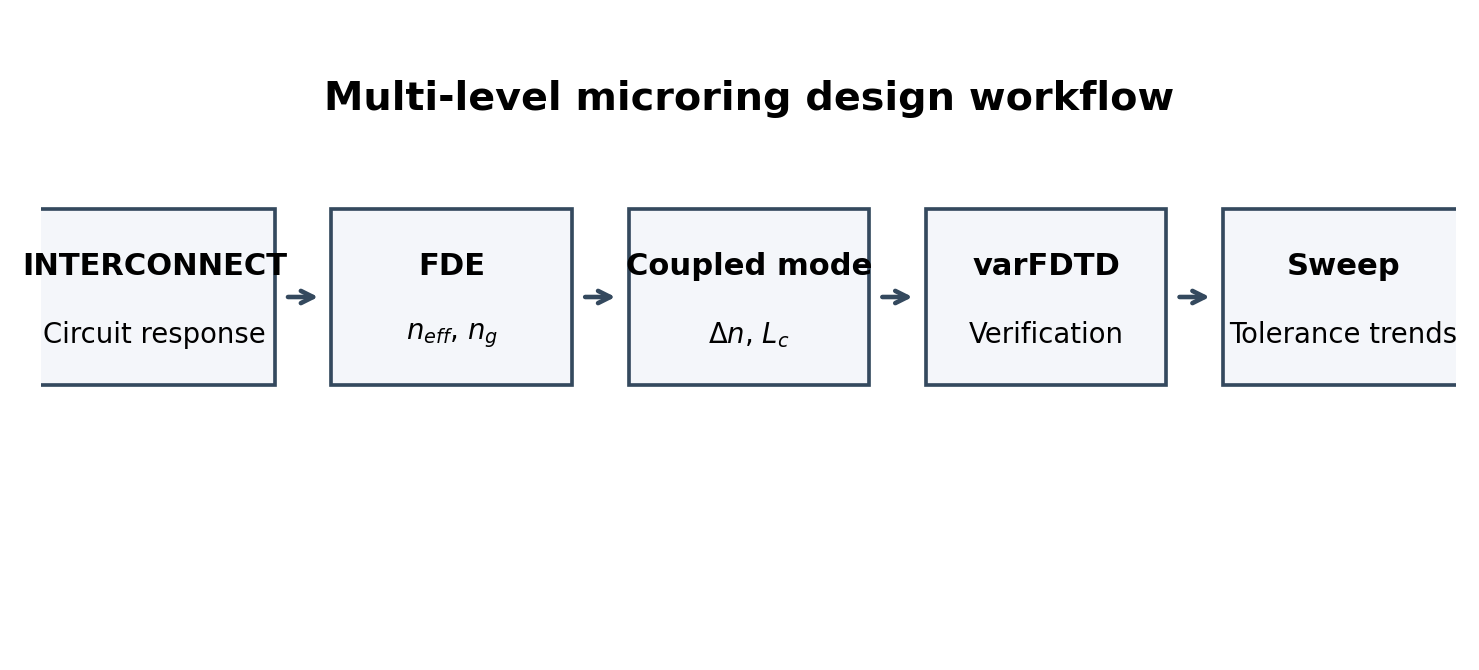
\includegraphics[width=0.92\linewidth]{figures/multilevel_workflow.png}
\caption{Conceptual multi-level workflow used for the report: system-level INTERCONNECT modelling, FDE modal extraction, coupled-mode design, varFDTD verification, and parameter sweeps.}
\label{fig:workflow}
\end{figure}

The original INTERCONNECT file \path{models_original/ring_resonator_student.icp} is available in the project directory but is not included in the Overleaf zip, following the requirement to avoid large Lumerical model files. No exported INTERCONNECT spectra or peak tables were found in \path{results/} or \path{figures/}. Therefore, Fig.~\ref{fig:workflow} is included only as a workflow schematic, not as a replacement for missing transfer functions.

\begin{table}[H]
\centering
\caption{INTERCONNECT quantities requested by the lab workflow. Missing entries should be filled after exporting ONA results from INTERCONNECT.}
\label{tab:interconnect-results}
\begin{tabular}{lll}
\toprule
Quantity & Value & Status \\
\midrule
Through-port transfer function & TODO & Not available from current simulation output \\
Drop-port transfer function & TODO & Not available from current simulation output \\
Resonance wavelength & TODO & Not available from current simulation output \\
FSR & TODO & Not available from current simulation output \\
FWHM & TODO & Not available from current simulation output \\
Drop-port \(Q\) factor & TODO & Not available from current simulation output \\
Drop-port finesse & TODO & Not available from current simulation output \\
Coupling coefficient & TODO & Not available from current simulation output \\
\bottomrule
\end{tabular}
\end{table}
